\documentclass[12pt]{article}
\title{EE445M Lab 7}
\author{Hershal Bhave (hb6279), Eric Crosson (esc625), \\
  and Matt Zhan (myz84)}
\date{Friday May 8, 2015}

\usepackage[in]{fullpage}
\usepackage{listings}
\usepackage{tabularx}
\usepackage{cleveref}
\usepackage[nosolutionfiles]{answers}
\usepackage{graphicx}
\usepackage{xcolor}
\usepackage{color}
\usepackage{enumerate}
\usepackage{pdfpages}
\usepackage{float}
\usepackage{subcaption}

\newenvironment{Ex}{\textbf{Problem}\vspace{.25em}\\}{}
\Newassociation{solution}{Soln}{Answers}
\pagebreak[3]
\newcommand{\Opentesthook}[2]{\Writetofile{#1}{\protect\section{#1: #2}}}
\renewcommand{\Solnlabel}[1]{\textbf{Solution}\quad}
\newcommand{\todo}[1]{{\color{red}{\LARGE TODO} #1}}
% \newcommand{\probb}{\textbf{Problem}\vspace{.25em}\\}
% \newcommand{\soll}{\\ \Solnlabel \newline \\}
\newcommand{\probb}{}
\newcommand{\soll}{\vspace{0.5em}\\}
\newcommand{\ohm}{$\Omega$}
\newcommand{\hbr}{\hfill\vspace{.25em}\\}
\newcommand{\dd}[1]{\:\mathrm{d}{#1}}
\newcommand{\ddt}[1]{\frac{\dd{}}{\dd{#1}}}
\newcommand{\dddt}[1]{\frac{\dd{}^2}{\dd{#1}^2}}

\definecolor{mygreen}{rgb}{0,0.6,0}
% \definecolor{mygreen}{rgb}{0.13,0.55,0.13}
\definecolor{mygray}{rgb}{0.5,0.5,0.5}
\definecolor{mymauve}{rgb}{0.58,0,0.82}

\lstset{
  backgroundcolor=\color{white},
  basicstyle=\scriptsize\ttfamily,
  breakatwhitespace=false,
  breaklines=true,
  captionpos=b,
  commentstyle=\color{mygreen},
  deletekeywords={...},
  escapeinside={\%*}{*)},
  extendedchars=true,
  frame=single,
  keywordstyle=\color{blue},
  rulecolor=\color{black},
  showspaces=false,
  showstringspaces=false,
  showtabs=false,
  stringstyle=\color{mymauve},
  tabsize=2,
  title=\lstname,
  columns=fullflexible,
}

\begin{document}
\maketitle

\section{Objectives}

\begin{itemize}
\item Design a robot that can move forward/backward, and turn left/right,
\item Interface motors, agnd sensors to two microcontrollers,
\item Implement pulse-width modulation using output compare to adjust power to the motors
\item Employ input capture interrupts to measure distance,
\item Write low-level device drivers for the motors and sensors,
\item Develop a high-level control system,
\item Use communication skills to work effectively as team.
\end{itemize}

\section{Hardware Design}

% \begin{figure}[H]
%   \centering
%   \begin{subfigure}[b]
%     % \includegraphics[width=\textwidth]{./img/mechanical-sketch.png}
%     \caption{Mechanical sketch of the robot}
%     \label{fig:mechanical-sketch}
%   \end{subfigure}
%   \begin{subfigure}[b]
%     % \includegraphics[width=\textwidth]{./img/motor-interface.png}
%     \caption{Electrical circuit diagram for the motor interfaces}
%     \label{fig:motor-interface}
%   \end{subfigure}
%   \begin{subfigure}[b]
%     % \includegraphics[width=\textwidth]{./img/motor-interface.png}
%     \caption{Power supply circuit}
%     \label{fig:power-supply}
%   \end{subfigure}
%   % \includegraphics[width=\textwidth]{./img/motor-interface.png}
%   \caption{Electrical circuit diagram for the sensor interfaces}
%   \label{fig:sensor-interface}
% \end{figure}

\section{Software Design}
Reference \cref{sec:code}.

\section{Measurement Data}
\begin{enumerate}
\item \probb Give the voltage and currents of each of the motors used.
  \soll The motors use 8.4 Volts at 100 mA at free-spinning/no-load.
\item \probb Give the robot speed and turning accuracy. \soll I don't know how
  to answer this question.
\item \probb Power supply current for various operations \soll Power
  supply current was between 150 and 400 mA during normal operation.
\item \probb Accuracy of the positioning system, knowing where it is
  \soll I don't know how to answer this question.
\item \probb Scores during qualifying and preliminary competition.
  \soll Reference \cref{tab:qualifier}.
  \begin{table}
    \centering
    \begin{tabular}{c|c}
      Qualifier Round & Score \\ \hline
      1 & 24 \\
      2 & 12 \\
      3 & 18 \\
    \end{tabular}
    \caption{Qualifier scores}
    \label{tab:qualifier}
  \end{table}
\end{enumerate}

\section{Analysis and Discussion}

\begin{enumerate}[1)]
\item \probb What is the effect of time delay in your control system?
  \soll The system responds more slowly.
\item \probb What sensors would you need to develop a more effective
  passing strategy? \soll In general, more sensors and more accurate
  sensors, Possibly GPS so that the robot would know another robot
  isn't a wall.
\item \probb If you hit the wall a lot, how could you have changed the
  design to be more effective? If your robot can travel 3 milestones
  without hitting a wall, you can skip this question. \soll Our robot
  can go three milestones without hitting a wall.
\end{enumerate}

\newpage
\section{Code}
\label{sec:code}
\lstinputlisting[language=C++,label=lst:motorcpp,caption=\texttt{motorpp.cpp}]{@doc-staging-area@/motorpp.cpp}
\lstinputlisting[language=C++,label=lst:motorhpp,caption=\texttt{motorpp.hpp}]{@doc-staging-area@/motorpp.hpp}
\lstinputlisting[language=C++,label=lst:switchcpp,caption=\texttt{switccpp.cpp}]{@doc-staging-area@/switchpp.cpp}
\lstinputlisting[language=C++,label=lst:switchpp,caption=\texttt{switchpp.hpp}]{@doc-staging-area@/switchpp.hpp}

\lstinputlisting[language=C++,label=lst:move,caption=\texttt{move-main.cpp}]{@doc-staging-area@/move-main.cpp}
\lstinputlisting[language=C++,label=lst:sense,caption=\texttt{sense-main.cpp}]{@doc-staging-area@/sense-main.cpp}

\begin{figure}[H]
  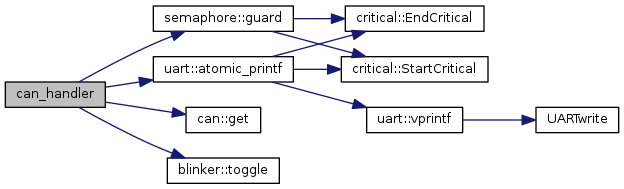
\includegraphics[width=\textwidth]{./img/motor_can_handler.png}
\end{figure}

\begin{figure}[H]
  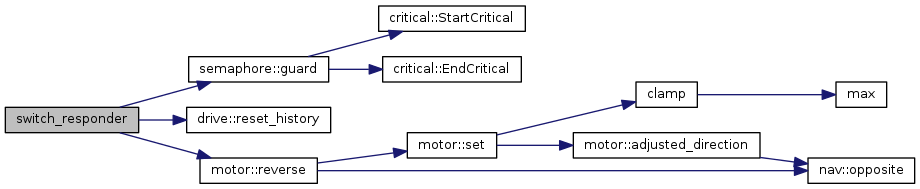
\includegraphics[width=\textwidth]{./img/switch_responder.png}
\end{figure}

\begin{figure}[H]
  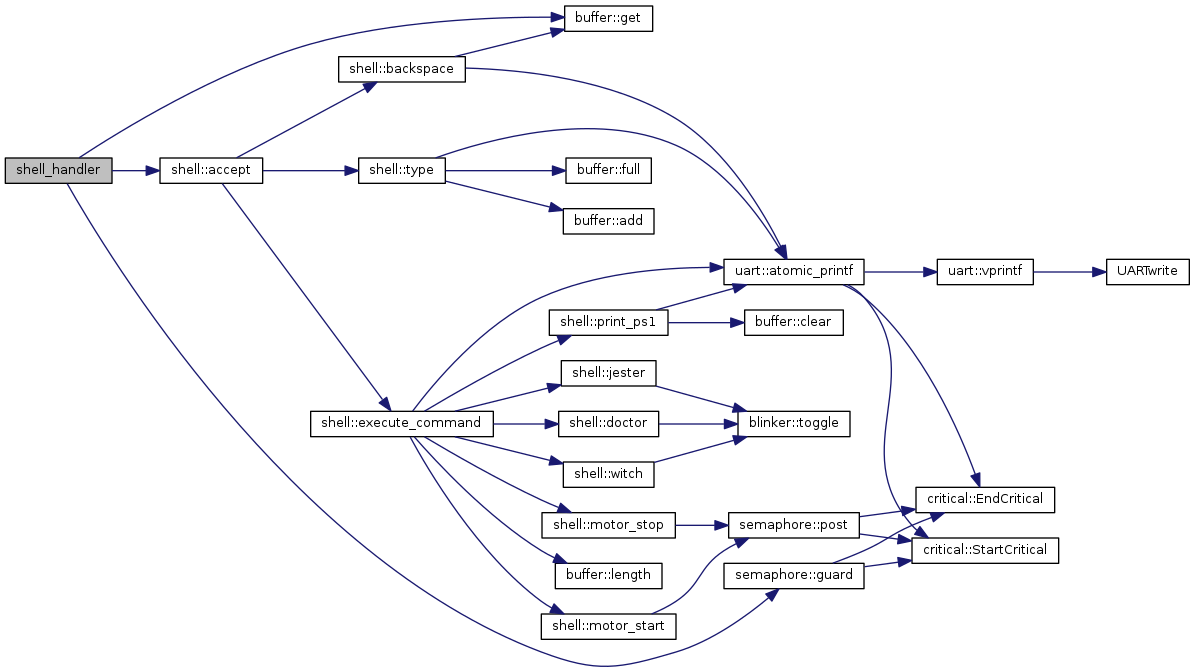
\includegraphics[width=\textwidth]{./img/shell_handler.png}
\end{figure}

\begin{figure}[H]
  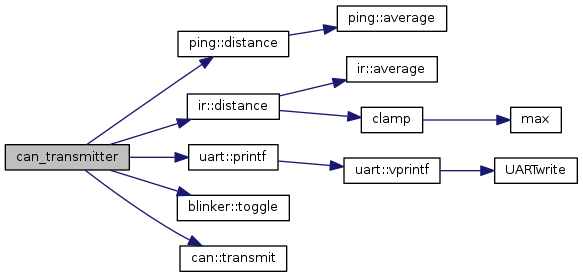
\includegraphics[width=\textwidth]{./img/sensor_can_transmitter.png}
\end{figure}

\begin{figure}[H]
  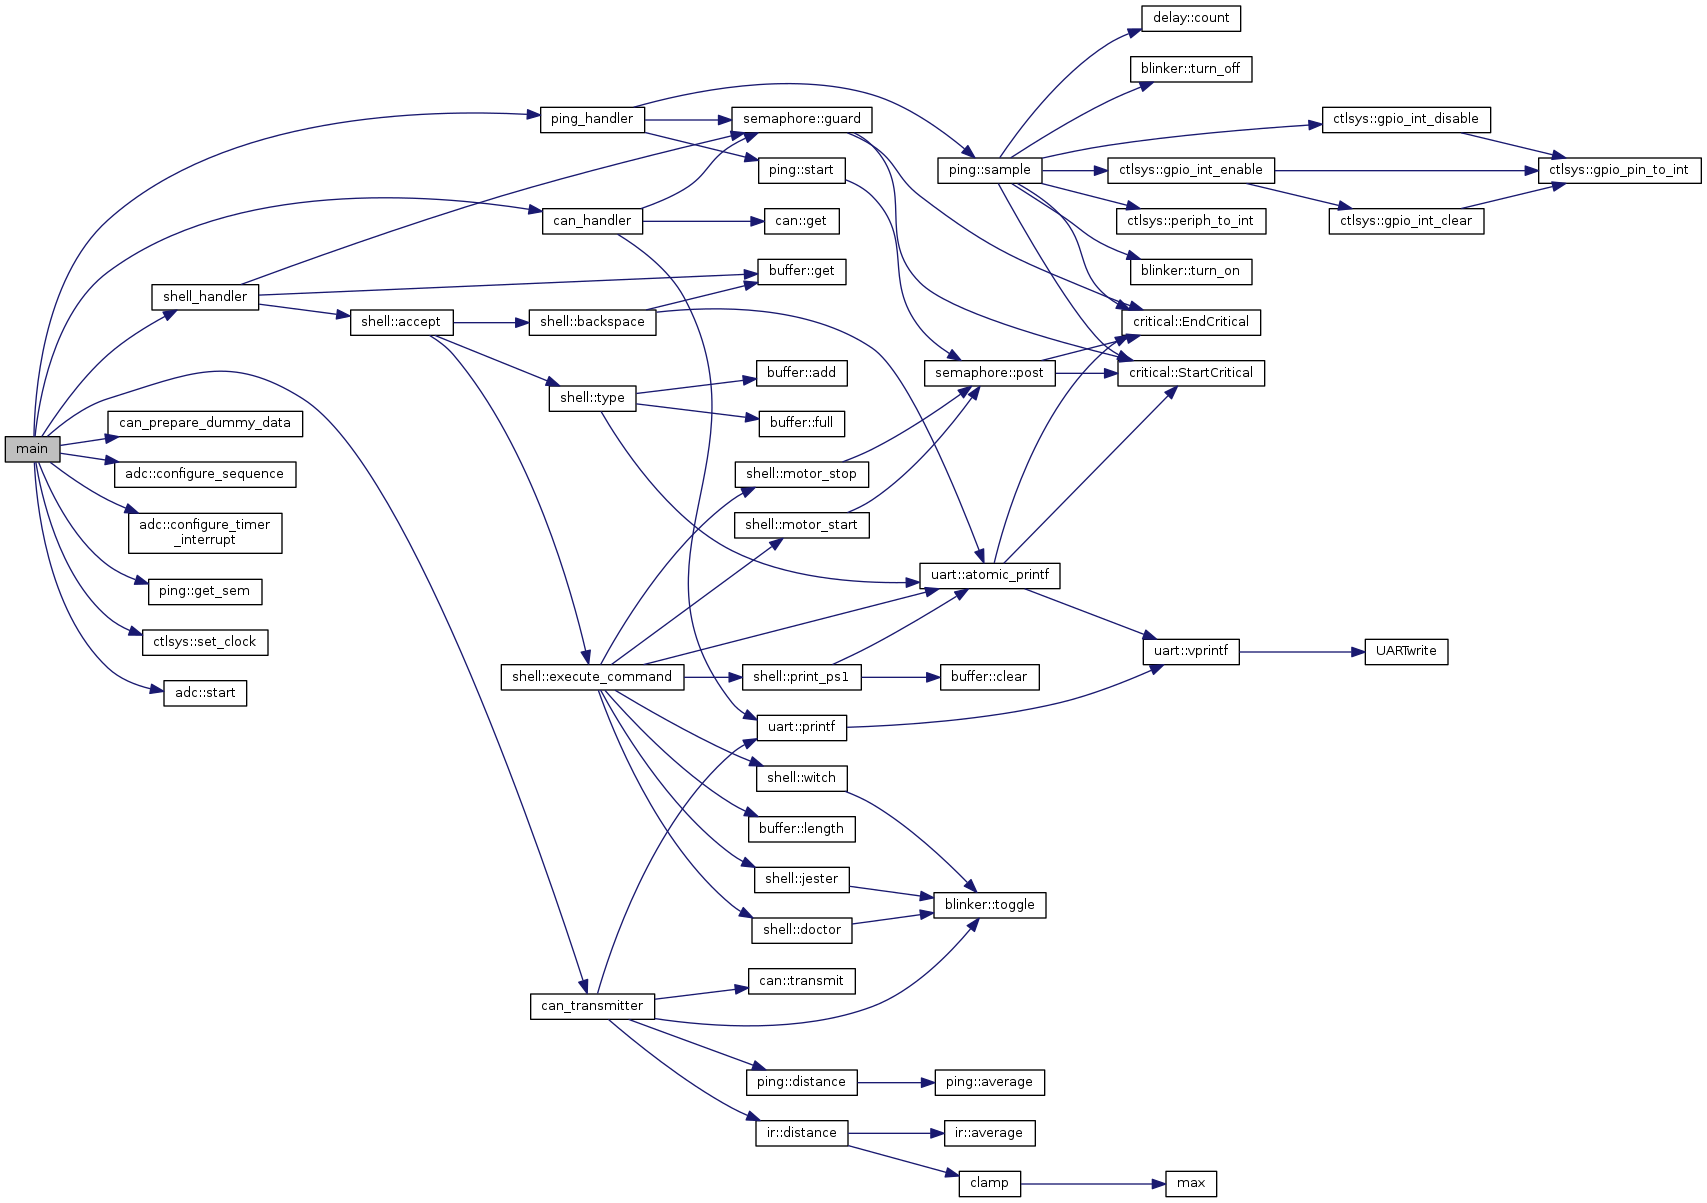
\includegraphics[width=\textwidth]{./img/sense_main.png}
\end{figure}

\begin{figure}[H]
  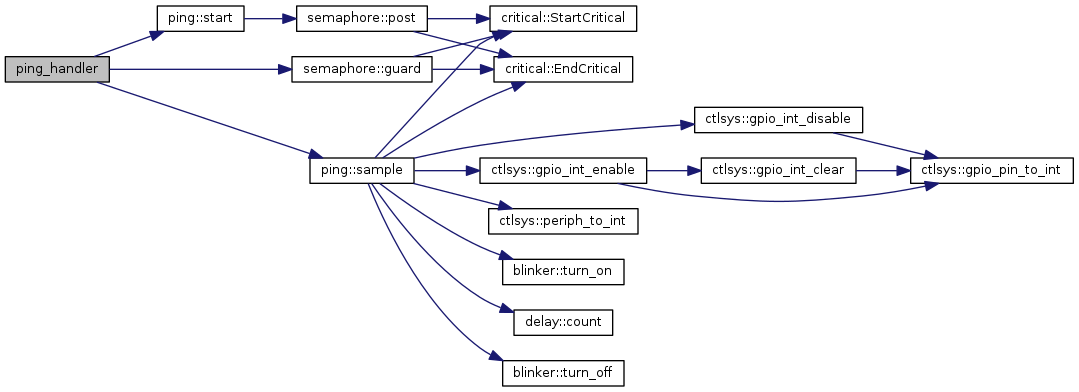
\includegraphics[width=\textwidth]{./img/ping_handler.png}
\end{figure}

\begin{figure}[H]
  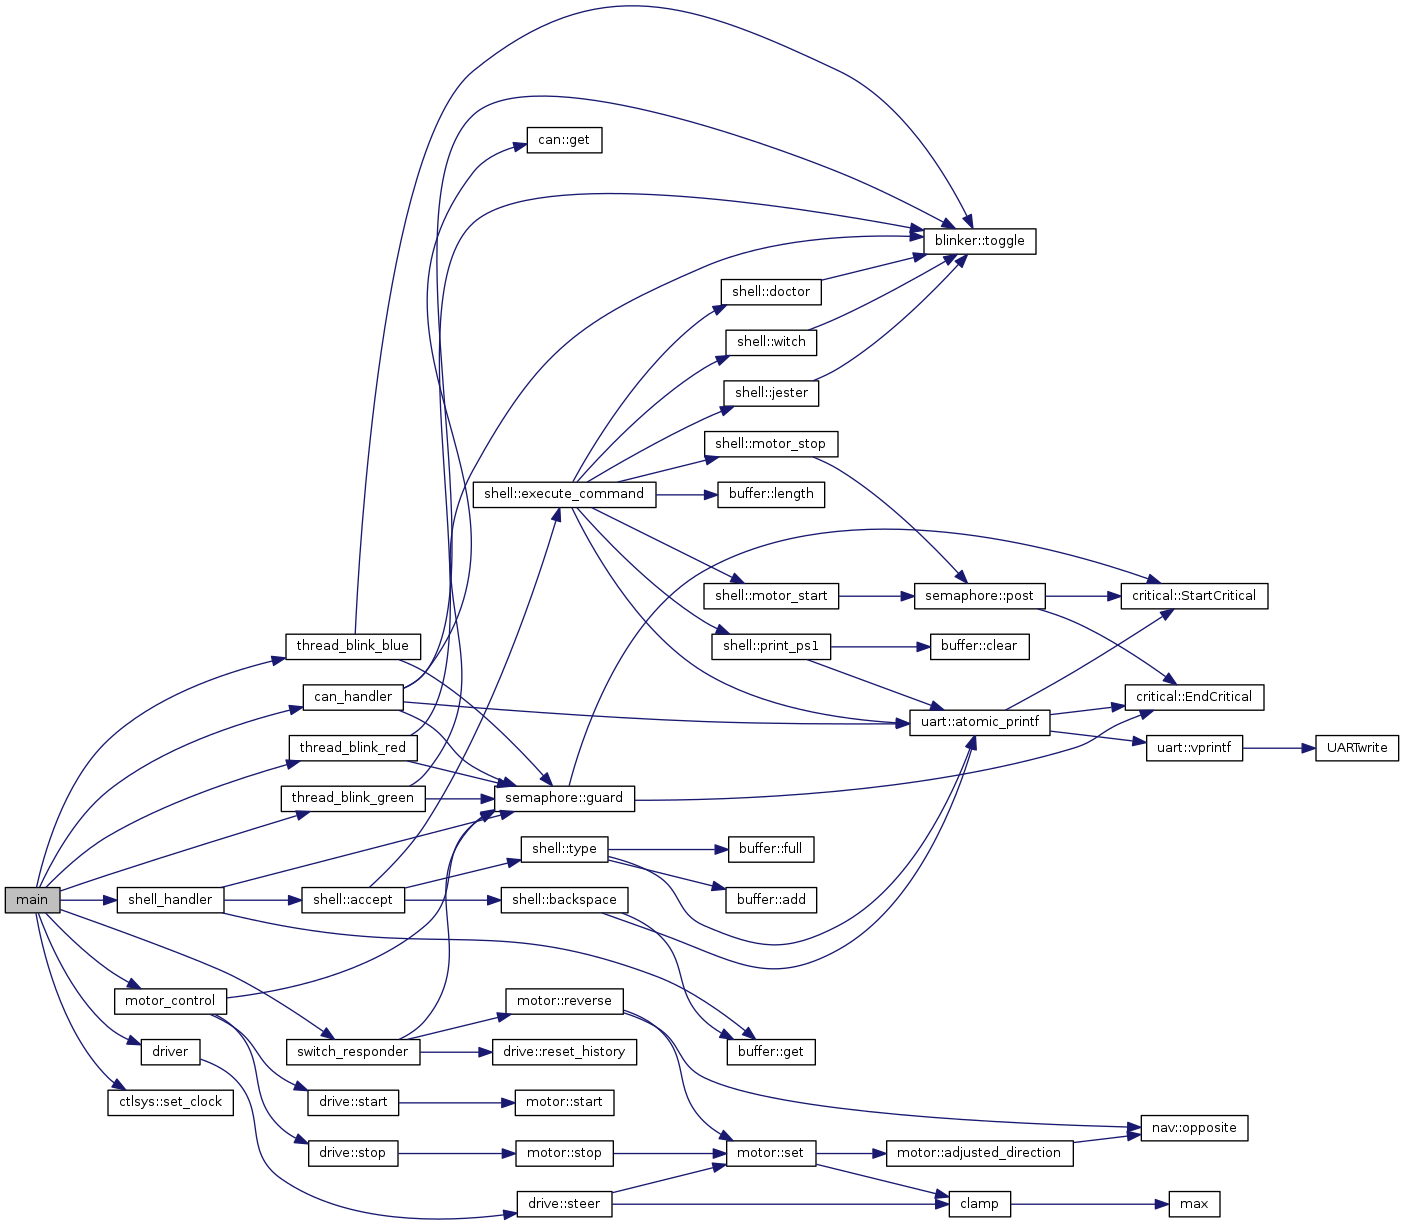
\includegraphics[width=\textwidth]{./img/move_main.png}
\end{figure}

\begin{figure}[H]
  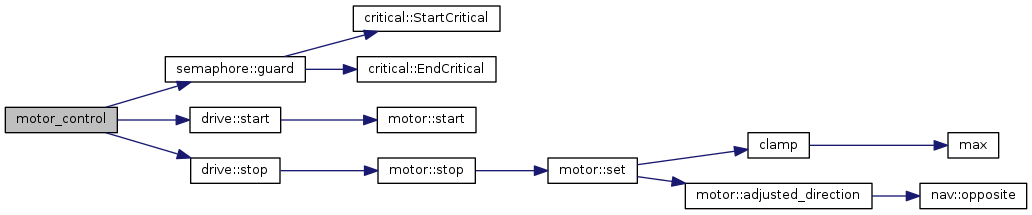
\includegraphics[width=\textwidth]{./img/motor_control.png}
\end{figure}

\end{document}
